\chapter{Phase Transitions and Critical Phenomena}
\label{ch2-crit}

%sources
    %Henkel - Conformal Invariance and Critical Phenomena - Ch1
    %Gitterman - Ch1
    %Nishimore - Ch1
    %Sole - Ch1

    %DIFFUSION-LIMITED GROWTH IN BACTERIAL COLONY FORMATION Mitsugu MATSUSHITA a
    %and Hiroshi FUJIKAWA b (LDA FIG)
    %http://people.umass.edu/machta/images/dla.html


A big part of the physics effort is to understand how the different components
of a system interact with one another. The actual identity of these components
depends on the context, they can be elementary particles when studying high
energy physics, atoms and molecules when studying the eletronic properties of a
material, living cells when observing the growing pattern of a colony of
bacteria, or even people when trying to design buildings with safe exit routes.

More often than not, these components can take many different patterns of
organization, which depend on the adjustment of some external parameter, like
energy density, temperature, nutrient concentration, or whether or not there is
a fire going on on the building. We call these arrangements \textit{phases},
and the global behavior of the system can have wildly different properties in
different phases despite having the same composition. Examples are abundant.
Anyone who has been through elementary school is familiar with the three
``standard'' phases of matter: solid, liquid and gas. When the temperature is
low enough, the cohesive forces between molecules dominates the dynamics of the
systems, locking them in place, giving rise to the solid state. When the
temperature is too high, thermal movement dominates and the particle are
basically free to move around. The liquid phase emerges in an intermediary
state, when the particles do not have to much energy to be fixes but not enough
to move freely.

Figure~\ref{fig:water}a shows the very famous phase diagram of water. It shows
in which phase the system is found for every value of pressure and temperature.
The black lines represent the border between each phase, when the control
parameters of the system (in this case pressure and temperature) change in a
way that crosses the boundary of a phase, the system undergoes a \textit{phase
transition}.

\begin{figure}
\begin{center}
    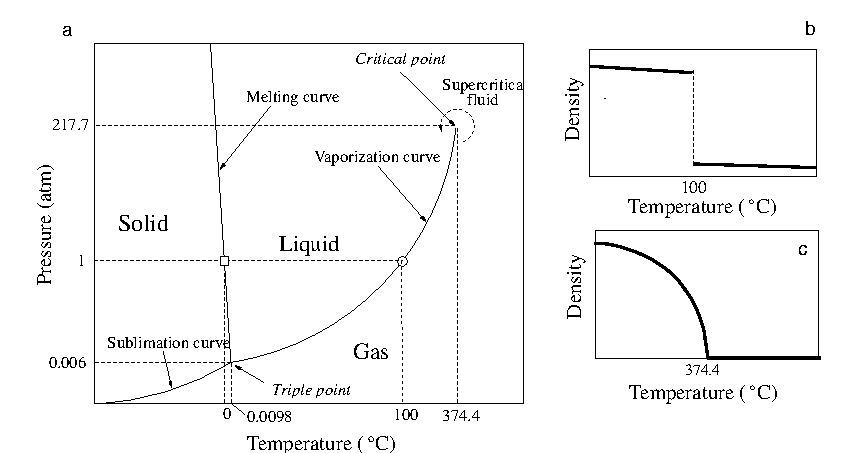
\includegraphics[scale=1.0]{chapters/ch2-crit/figs/water}
\end{center}
\caption{Phase diagram of water (a). Here, the three usual phases are
    distinguished, each separated from the other by a critical line. The phase
    transition that happens when the system traverse a line is characterized by
    a discontinuous jump in the density, as shown in (b) for the liquid-gas
    transition at $P=1$ atm. For $P=217.7$ atm however the same transition is
    continuous, as shown in (c). In the vicinity of this phase transition, at
    $T\approx374.4^\circ$C, the two phases become indistinguishable, and
    display a number of peculiarities. Systems in such state are called
    critical systems. Reproduced from [???].}
% taken from Sole - page 7
\label{fig:water}
\end{figure}

Below we present two important models in the study of phase transition
Figure~\ref{fig:water} 


\section{Ising Model}
\label{sec:ising}

The Ising model represents the golden standard of phase transition models
because it unites a quite simple physical description with the fact it can be
exactly solved in both one and two dimensions, a claim very few models can
make.

The system is composed of a number of classical spins $\{s_i\}$ that can take
one of two values $1$ or $-1$. The are arranged in a lattice and are allowed to
interact with its first nearest neighbors. The Hamiltonian of the systems is
given by
\begin{equation}
    \label{eq:ising}
    H\left(\left\{s_{i}\right\}\right) = 
        -J\sum_{\left\langle i,j\right\rangle}s_{i}s_{j}
        -h\sum_{i}s_{i}.
\end{equation}
Where $\sum_{\left\langle i,j\right\rangle}$ means a summation over all pairs
of nearest neighbors. If we assume $J>0$, then the first term of the
Hamiltonian favors the alignment of the spins, while the second one 
favors the alignment with an external magnetic field.

Just like the water example, the phase diagram of the Ising model is dependent
on two variables: the external magnetic field $h$ and the temperature $T$.

\begin{figure}
\begin{center}
    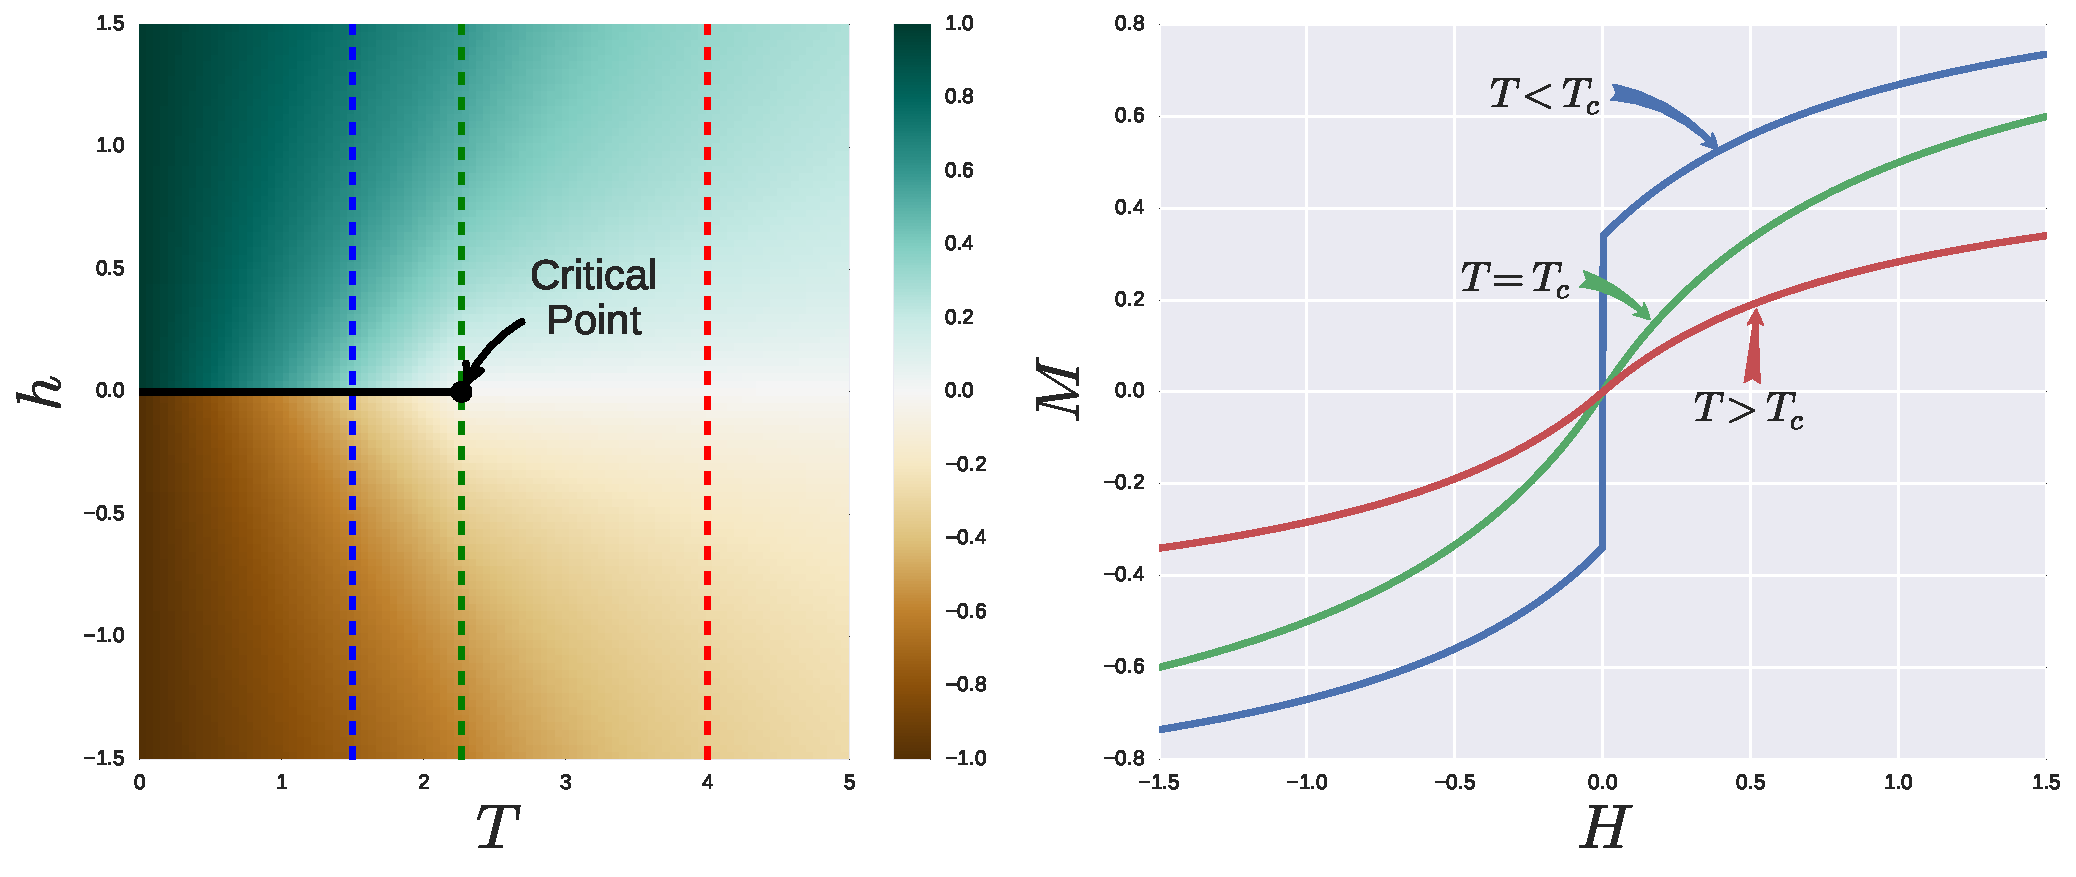
\includegraphics[scale=0.4]{chapters/ch2-crit/figs/ising_phase2}
\end{center}
\caption{The phase space of the Ising model (left). The color represents the
    spontaneous magnetization $M$ as a function of the external magnetic field
    $h$ and temperature $T$. The black line represents the critical line where
    the phase transition is of first order, which means the magnetization
    changes discontinuously like it's shown in the blue line. In the critical
    point the change is continuous and a second order phase transition takes
    place. Above the critical point no phase transition takes place.}
\label{fig:ising_phase2}
\end{figure}


\begin{figure}
\begin{center}
    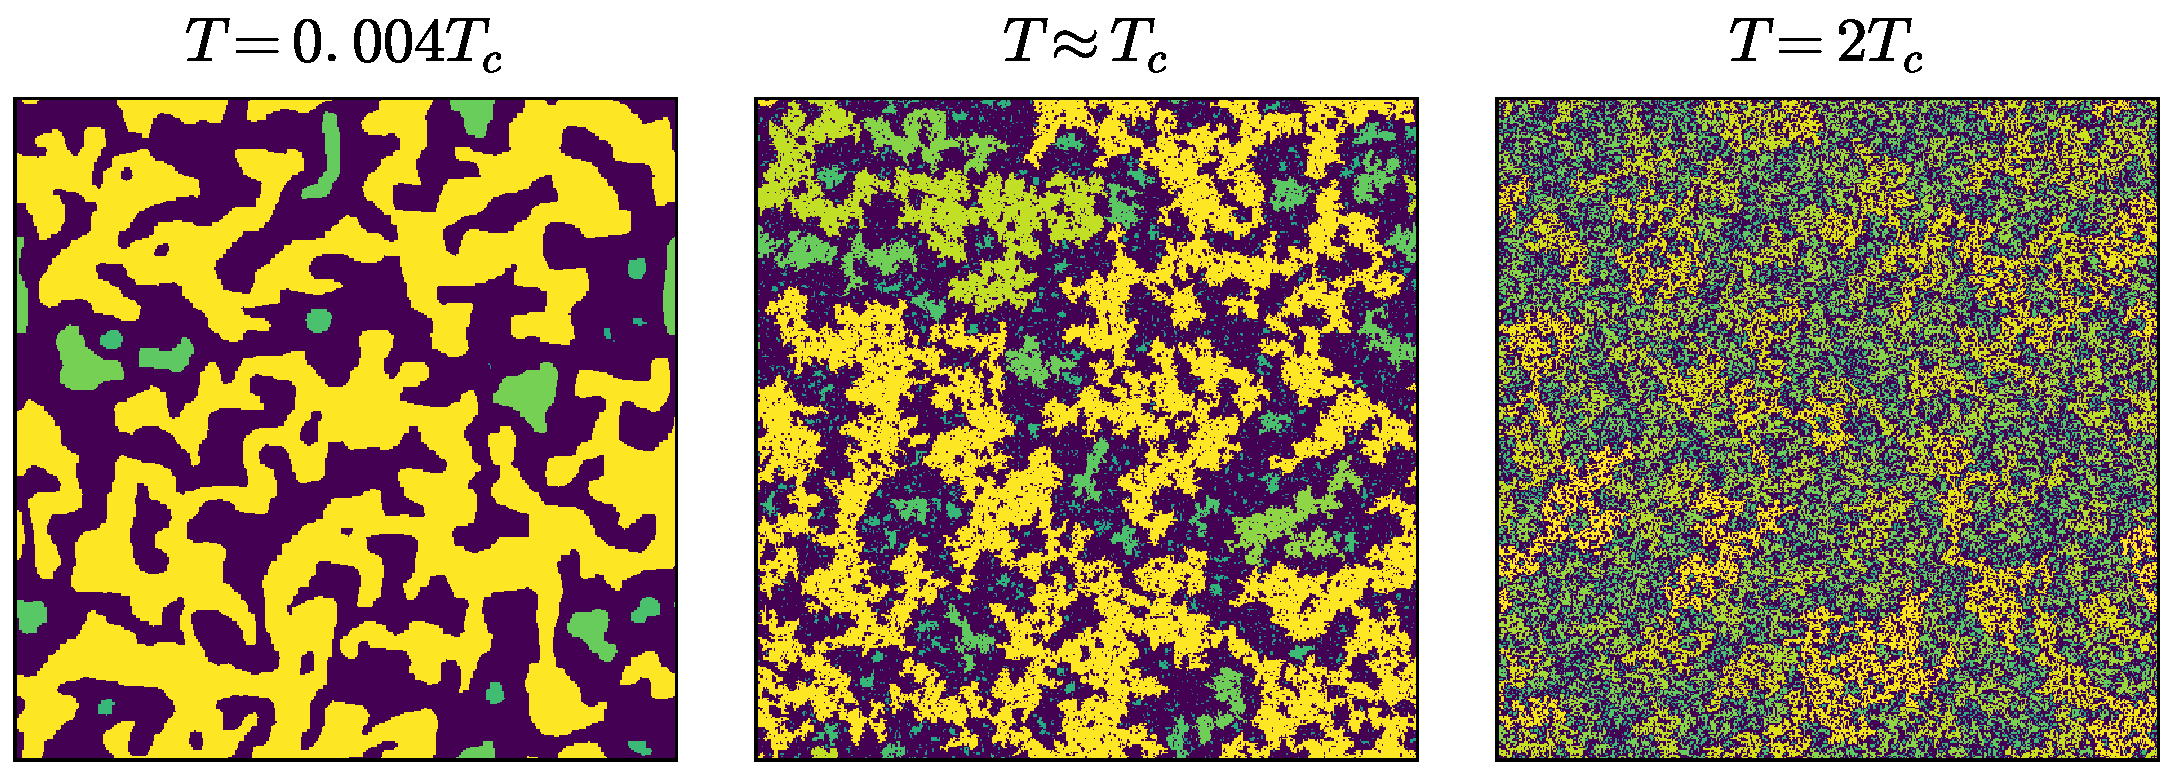
\includegraphics[scale=0.4]{chapters/ch2-crit/figs/ising}
\end{center}
\caption{Realizations of the Ising model with three different
    temperatures. The clusters of adjacent spin-up sites are colored according
    to how many sites belong to it. The subcritical regime is dominated by the
    large clusters. On the other hand, above the critical point, the system is
    dominated by thermal fluctuations, undermining cluster formation. At the
    critical point however, the clusters lack a characteristic length scale.
    One can observe that the image has a certain ``depth'' to it. This happens
    because clusters of all sizes are present, a mark of scale invariance,
    the most important property of critical systems.}
\label{fig:ising}
\end{figure}

\begin{figure}
\begin{center}
    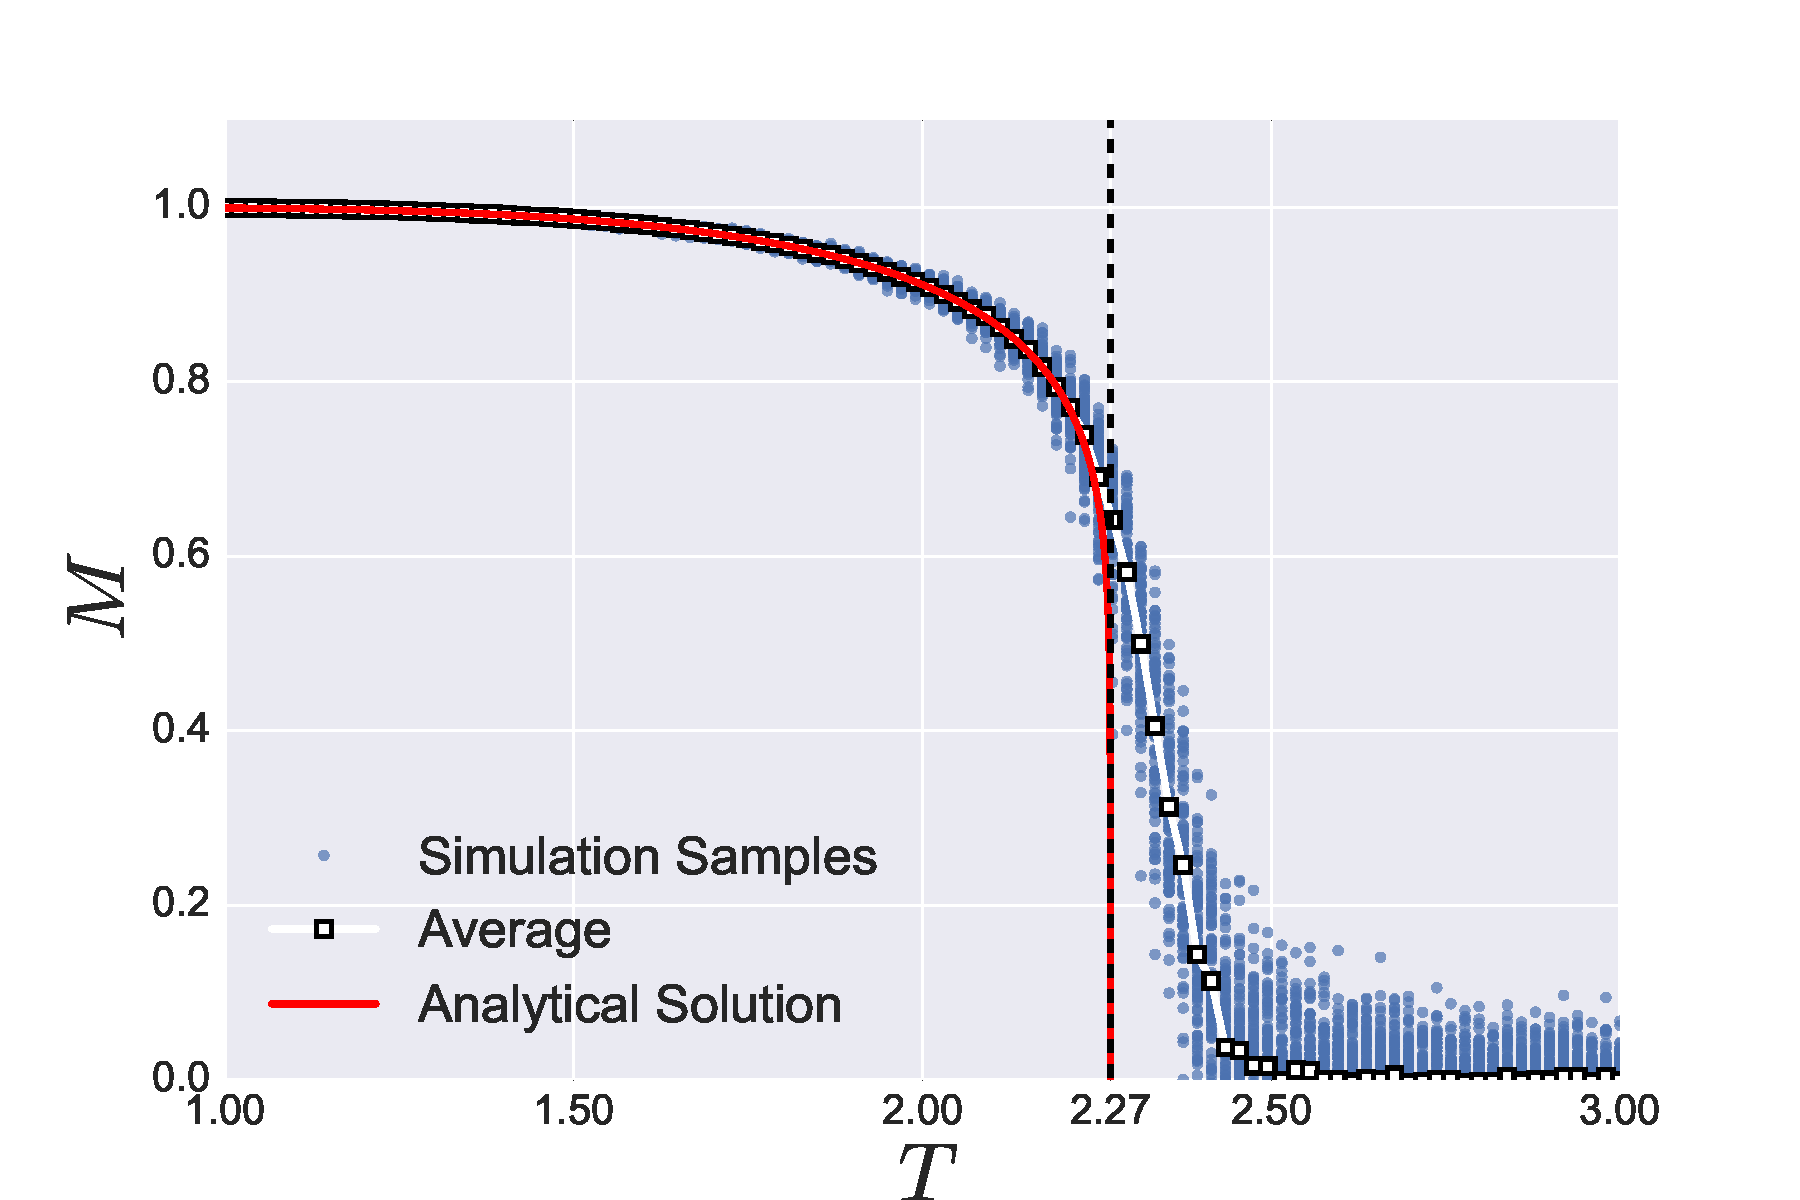
\includegraphics[scale=0.4]{chapters/ch2-crit/figs/ising_phase}
\end{center}
\caption{Spontaneous magnetization as a function of temperature for the Ising
    model. The simulations were performed in a $128\times128$ square lattice.
    As temperature rises, thermal fluctuations dominate the spin dynamics
    destroying the correlations. Above the critical temperature of
    $T_c=2/\log(1+\sqrt{2})\approx 2.269$ the value of $M$ should reaches zero,
    although due to finite size effects we still observe some magnetization
    beyond this point. The red line shows the illustrious solution
    developed by Onsager, where $M=[1-(\sinh{2/T})^{-4}]^{1/8}$.}
\label{fig:ising_phase}
\end{figure}


\section{Percolation}
\label{sec:perc}

While the Ising model certainly wins in terms of popularity, very few models
match the simplicity of percolation. Introduced in 1957 by Broadbent and
Hammersley, the passing decades saw its rise in prominence due to it's high
applicability ranging from transport in porous media to the propagation of
infectious diseases, with pretty much everything in between.

The original question Broadbent and Hammersley posed when coming up with
percolation was as fallows: if we submerge a large porous rock in water, will
the water penetrate the rock all the way to its center? In order to answer this
question they proposed the following model. We take a square lattice in any
number of dimensions wanted; this will be our rock.

\begin{figure}
\begin{center}
    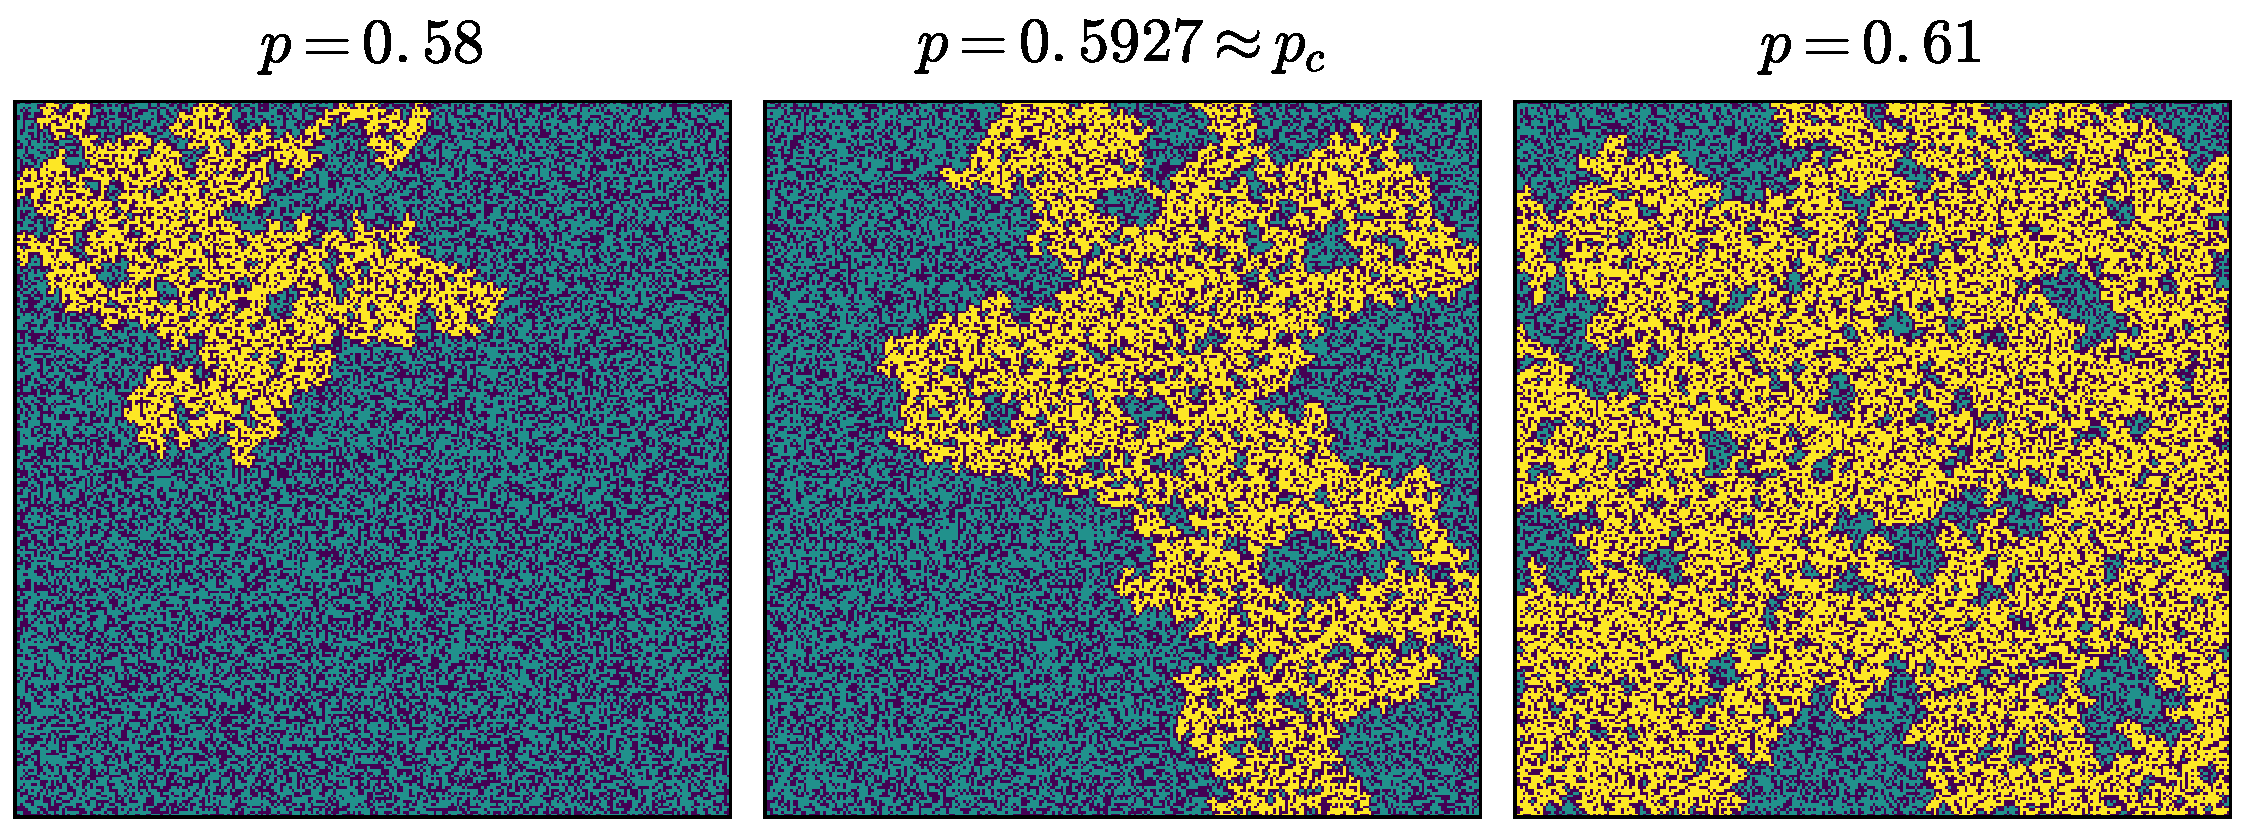
\includegraphics[scale=0.4]{chapters/ch2-crit/figs/isoperco}
\end{center}
\caption{Realizations of the percolation model in a square lattice with three
    different occupation probabilities $p$. Black sites are unoccupied, blue
    ones are occupied, and the largest cluster is painted yellow. For small
    values of $p$, there is no cluster that connects opposite sides of the
    systems. Above the critical point however, the largest cluster promotes a
    global connectivity, or, in terms of transport, the system becomes
    permeable.}
\label{fig:isoperco}
\end{figure}

\begin{figure}
\begin{center}
    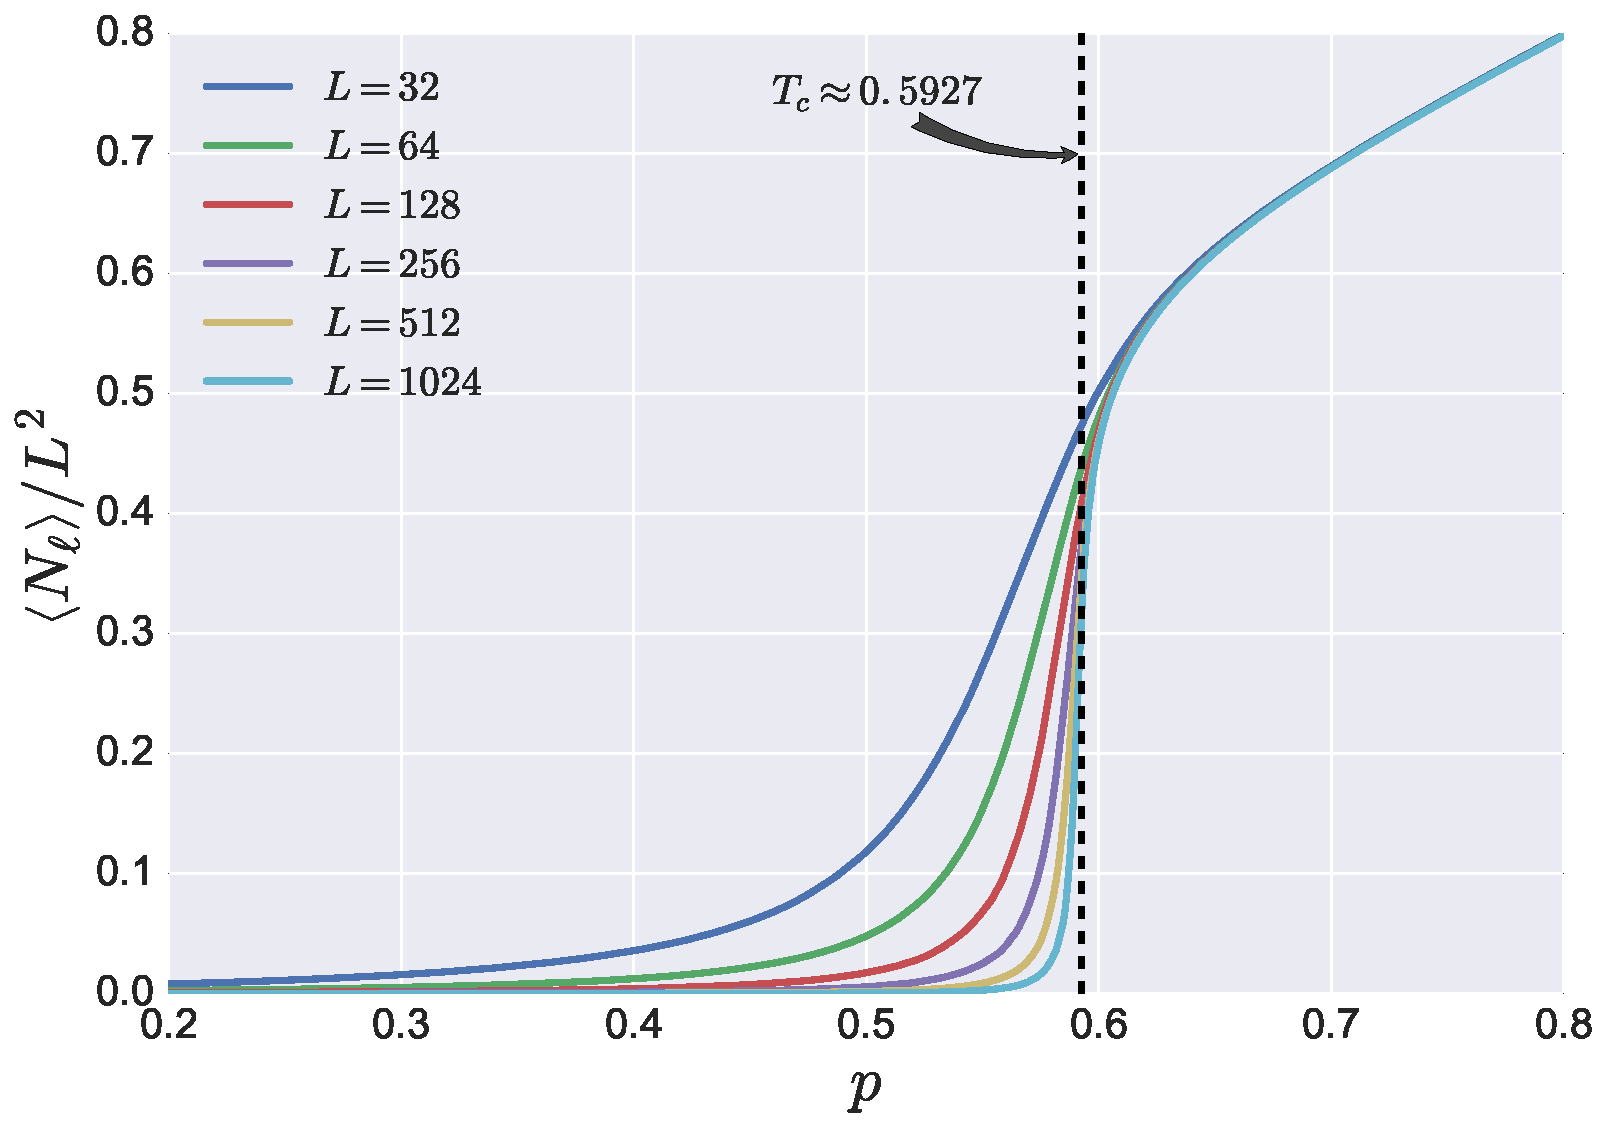
\includegraphics[scale=0.4]{chapters/ch2-crit/figs/isoperco2}
\end{center}
\caption{The order parameter of the percolation model as a function of the
    occupation probability for various system sizes. The order parameter here
    is defined as the fraction of the system occupied by the largest cluster.
    In the thermodynamical limit, the largest cluster have a finite size for
    $T<T_c\approx 0.592746$, that is, it occupies a negligible fraction of the
    system. Above the critical point the largest cluster is infinite and occupies
    a finite fraction.}
\label{fig:isoperco2}
\end{figure}

%\begin{figure}
%\begin{center}
    %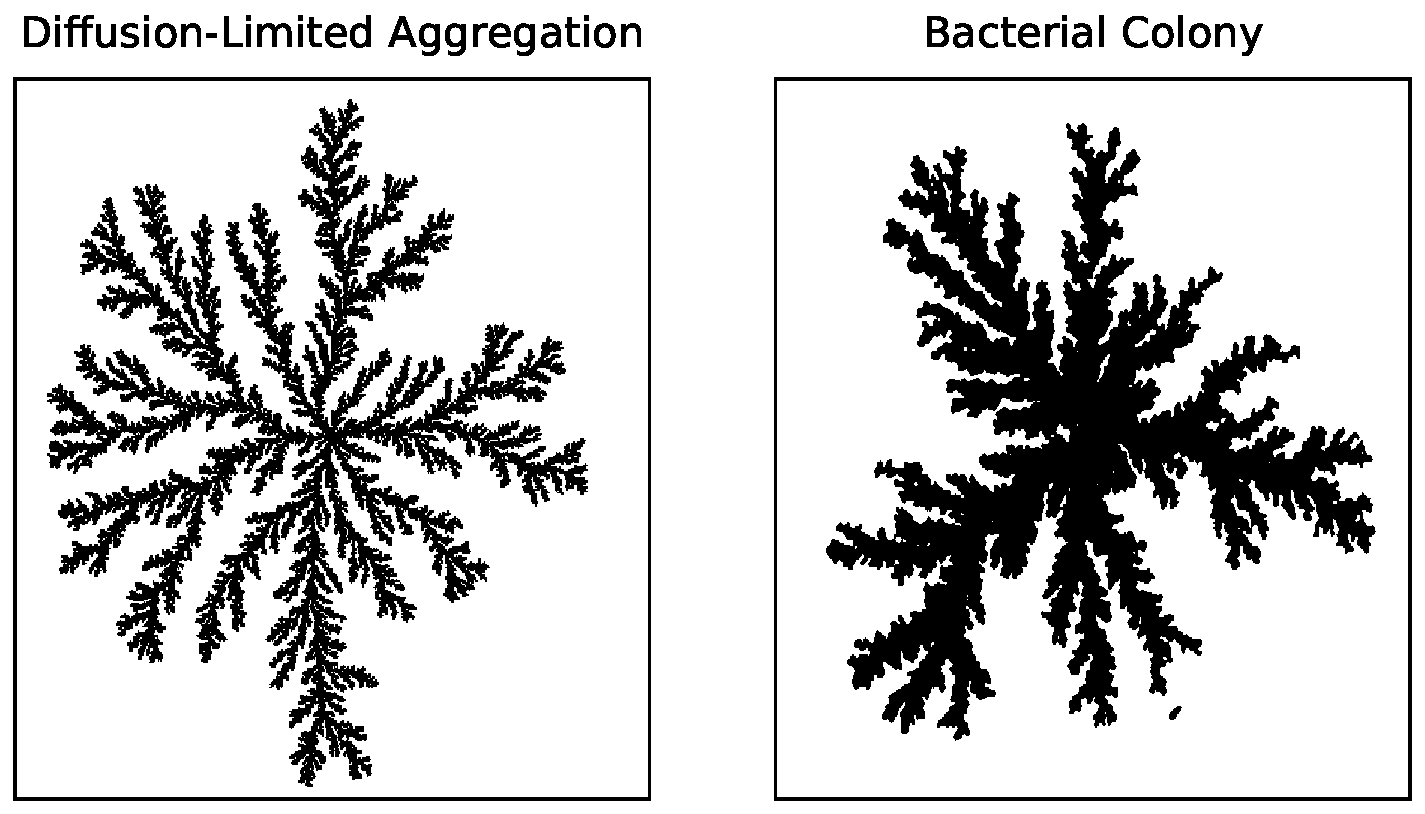
\includegraphics[scale=0.6]{chapters/ch2-crit/figs/bacteria}
%\end{center}
%\caption{Images taken from [???] and [???].}
%\label{fig:bacteria}
%\end{figure}
